\chapter{Background technologies}
In today's rapidly evolving digital landscape, the demand for simple and flexible software production technologies has become crucial. 
Virtualization and containerization emerged as a response to this need, gaining affirmation as fundamental complexity-enabler assets in the field of software engineering.
Among them, Docker containers made software deployment transition from monolithic to microservices architectures, paving the way for the widespread adoption of DevOps practices. 

This chapter aims at providing a brief overview about these technologies, their history and why they have revolutionized the software production landscape.
\newpage

\section{Historical perspective}
Software development and deployment are the two main software production processes at the core of software engineering. Together, they encompass all the activities required to design, code, test, install, configure and maintain a software product. In a nutshell, software development and deployment can be considered as the two macro-phases of the software production lifecycle. As macro-phases, they are made of several sub-phases, each one with its own set of activities, models and paradigms.
More specifically, the term "software development" refers to all the phases that lead to the creation of a software product, namely system and software requirements definition, requirement analysis, program design, coding and testing. The term "software deployment" encompasses all the steps that are necessary to make a software product available to its end users, such as software installation, configuration and maintenance. 
Despite historically considered as separate and managed by different production teams (development and operations), these two processes have always been deeply interconnected, defining and feeding the digital revolution since its dawn.

The diffusion of the first software production techniques dates back to the late 1950s, with the creation of the FORTRAN programming language.
Initially, software production followed the example set by other engineering disciplines, such as electronics, aerospace or even construction engineering. Software was developed in a monolithic fashion and deployed on mainframes, usually time-shared among several users. 
The two software production macro-phases, development and deployment, were clearly separated: software was produced following a structured and sequential approach, as in a production line. Several teams were involved in the process, each one responsible for a specific development and deployment sub-phase.  
This approach emerged as a common practice with the diffusion of vast software projects and was formalized in the Waterfall model, introduced by Winston Royce in 1970 \cite{royce1987managing}.
Despite being the first formal definition of a software production methodology, the Waterfall model emerged soon as too rigid and poorly adaptable to changes in software requirements due to limited feedbacks between the various production phases.

Over time and with the evolution of the digital world towards new needs and greater complexity, new production paradigms have become necessary to favor greater flexibility and adaptability to changes in software requirements. 
This necessity became an open problem, during what is still remembered as the past century software crisis: software projects were often late, exhibited poor quality and failed to meet functional and budget requirements.
In this scenario, the 1968 NATO Software Engineering Conference, held in Garmisch, Germany, is considered the milestone that gave birth to software engineering as a formal, self-standing discipline in the engineering landscape \cite{nato1968}.

\newpage
At the end of the past century, the widespread adoption of both new and mature technologies and paradigms completely re-shaped the software production landscape. From the development standpoint, the Waterfall model was limited to critical and real-time projects, giving way to more flexible development methodologies on the commercial side, such as spiral \cite{boehm1988spiral}, RAD (Rapid Application Development) \cite{martinRapidApplicationDevelopment1991} and Agile \cite{ManifestoAgileSoftware}. 
From the deployment standpoint, the diffusion of Internet and Linux-based virtualization technologies allowed the creation of remote server networks, giving birth to new cloud-based models, such as Software as a Service (SaaS), Platform As a Service (PaaS) and Infrastructure as a Service (IaaS) \cite{manvi2014resource}. With the flourishing of cloud computing, the monolithic deployment model was gradually abandoned in favor of more flexible and scalable architectures. This trend was further accelerated by the diffusion of containerization technologies:  applications began to be deployed as a set of isolated, loosely coupled microservices, communicating through APIs and hosted on cloud-based, multi-tenant environments.
This result was achieved at the end of a long journey, started in 1979 with the introduction of the \texttt{chroot} system call \cite{kerriskLinuxProgrammingInterface2010} during UNIX Version 7 development. FreeBSD Jails \cite{kampJailsConfiningOmnipotent}, Solaris Zones \cite{priceSolarisZonesOperating2004} and Linux Containers \cite{LinuxContainers} are the most relevant milestones towards the creation of modern container-based process isolation techniques.

Nowadays, Docker is the de facto standard for containerization. It was introduced on March 15, 2013, by Solomon Hykes, founder and CEO of a PaaS company called dotCloud, during the annual Python Developers Conference in Santa Clara, California \cite{hykesLightningTalkFuture2013}. Docker was an immediate success: the project's source code was released on GitHub as open-source, quickly gaining the attention of the software development community.
In 2013, dotCloud focused its efforts on the development and support of the Docker project, changing its name to Docker Inc. In June 2015, the Open Container Initiative (OCI) \cite{OpenContainerInitiative} was founded by the major key players in the container industry with the goal of creating open industry standards.

Over the last decade, Docker has radically changed the way software is developed and deployed on the cloud. By promoting the adoption of microservices, it fostered the transition from traditional software engineering to DevOps practices: development and operations teams are not strictly separated anymore, but work closer with the goal of improving software quality and delivery speed.
To achieve this goal, software development and deployment have become even more connected and automated: pipelines of Continuous Integration and Deployment (CI/CD) have become simpler, allowing production teams to test and release the software faster. 
Besides the benefits, the adoption of Docker containers has also brought new security challenges and risks, especially regarding container isolation in multi-tenancy cloud deployments \cite{luo2016whispers,gao2018study}.
These problems gave birth to container security as a new cybersecurity field and are still the subject of active research.

\section{Linux operating system architecture}
By being open-source, highly performant and secure, 
Linux is by far the most popular operating system in the server market. The diffusion of virtualization and containerization technologies boosted its adoption for enterprise solutions, making it the OS of choice when deploying applications in cloud environments.

Figure \ref{fig:linux_os_structure} provides a high-level overview of the Linux OS architecture.
Starting from the top of the diagram, users interact with the operating system though the user interface layer, which includes Graphical User Interfaces (GUIs), Command Line Interfaces (CLIs) and batch interfaces. GUIs provide elements for user visual interaction, such as windows, icons, buttons and menus. CLIs implement the command-based user interaction by allowing users to launch commands and scripts. Batch interfaces allow users to schedule command execution at specific times or conditions.
The user interface layer is the outermost user space layer and allows users to interact with both system and installed applications.
The term "user space" refers to the memory area where unprivileged user applications are run. 
User space applications are said to be running in "user mode", meaning they have constrained access to system resources and are prevented from executing critical operations that could compromise system's stability and security. \newline
Right below the user interface layer, shell interpreters connect CLIs and batch interfaces to the application layer by interpreting and executing commands.
The application layer includes both system and user-installed applications, running in user mode. Right below this layer, the process layer includes all active user processes, namely all instances of running applications. System libraries are shared among all processes and provide a high-level programming interface to kernel functionalities. 
Below system libraries, the diagram depicts the kernel space, namely the memory area that hosts the operating system kernel and its modules. 
The kernel is the software component that acts as the core of the operating system, handling the vast majority of critical tasks such as process scheduling, memory and filesystem management, I/O operation handling and security enforcement.
Kernel space software runs in "kernel mode", meaning it has full access to system resources and can execute privileged operations.
The first kernel space layer, namely the system call interface, provides an abstraction layer between user and kernel space. It allows user processes - running in user mode - to access kernel functionalities in a secure and predefined way.
At the lowest level, architecture-dependent kernel code allows the kernel to interact with the underlying hardware, including all the host physical components.

\begin{figure}[htbp]
    \vspace{10pt}
    \centering
    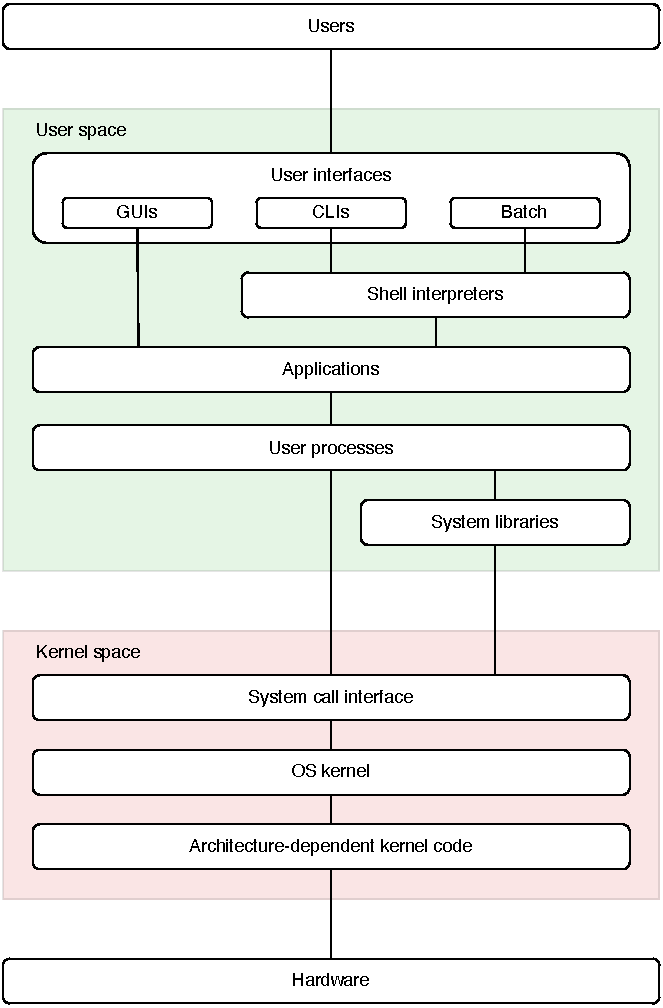
\includegraphics{assets/linux_os_structure.pdf}
    \caption{Linux OS architecture}
    \label{fig:linux_os_structure}
    \vspace{10pt}
\end{figure}

\section{Traditional application deployment}
Before the diffusion of virtual machines and containers, software deployment was a time-consuming process involving several steps and a lot of communication efforts between IT development and operations teams. 
This complexity posed big limits to innovation, reducing software delivery speed and quality: if deploying new software is hard, developers may be tempted to avoid solving problems that require new development efforts \cite{kaneDockerRunningShipping2023}.
The discussion that follows complements figure \ref{fig:traditional_deployment} in describing an old-fashion software deployment pipeline.
\begin{enumerate}
    \item Developers request available deployment resources to the operations team, specifying application requirements.
    \item Resources are set up and provisioned by the operations team.
    \item Developers script the deployment process, including application configuration and dependencies installation.
    \item Operations engineers and developers tweak the deployment script until the application is deployed as expected in a testing environment.
    \item Necessary changes in the application deployment are discovered by developers, such as new configuration parameters or additional dependencies. 
    \item The operations team work to fullfil the new deployment requirements.
    \item Steps from 4 to 6 are repeated as needed.
    \item The application is deployed to production environments.
\end{enumerate}

\begin{figure}[htbp]
    \vspace{10pt}
    \centering
    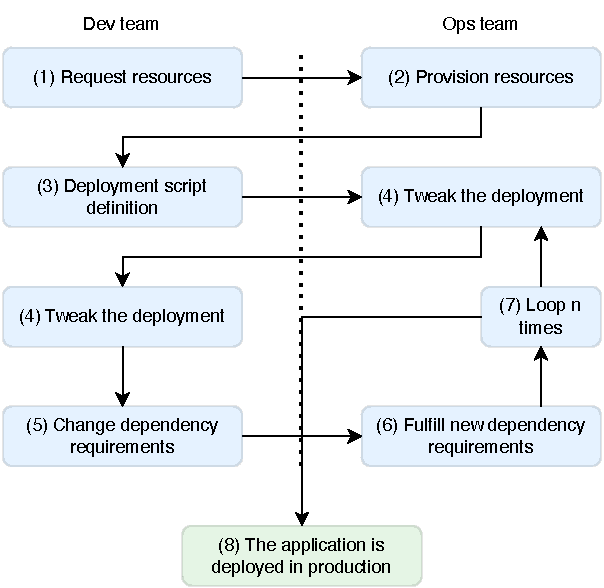
\includegraphics{assets/deployment_traditional.pdf}
    \caption{Application deployment before virtual machines and containers}
    \label{fig:traditional_deployment}
    \vspace{10pt}
\end{figure}

\section{Virtualization technologies}
Virtualization technologies emerged as the first solution to the deployment problem by creating strictly isolated environments (Virtual Machines or VMs) on the same physical hardware. 
Each VM consists in a full-fledged OS instance, with its own kernel and user space.
The software layer responsible for assigning physical resources to VMs is called hypervisor.
Depending on the hypervisor collocation, virtualization technologies can be divided into two main categories: bare metal (type 1) and type 2. 

\begin{figure}[htbp]
    \vspace{10pt}
    \centering
    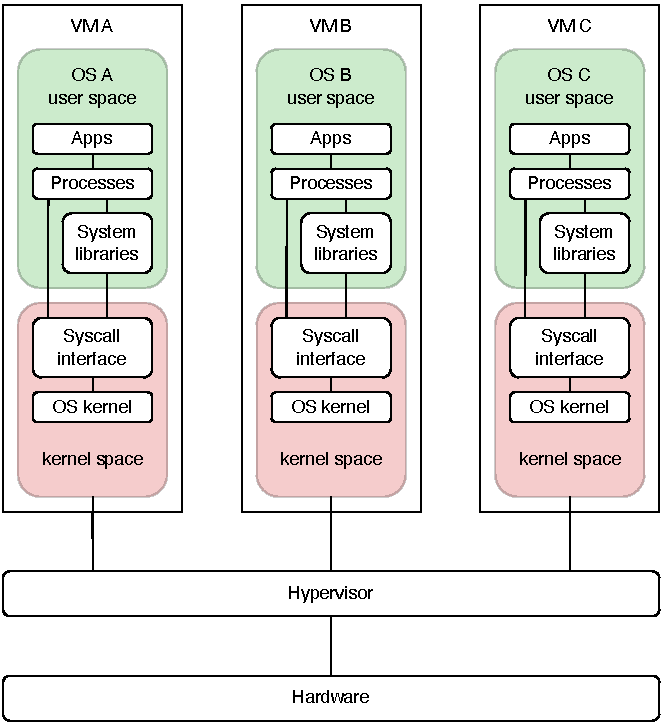
\includegraphics{assets/type_1_virtualization.pdf}
    \caption{Bare metal (type 1) virtualization environment}
    \label{fig:bare_metal_virtualization}
    \vspace{10pt}
\end{figure}

\begin{figure}[htbp]
    \vspace{10pt}
    \centering
    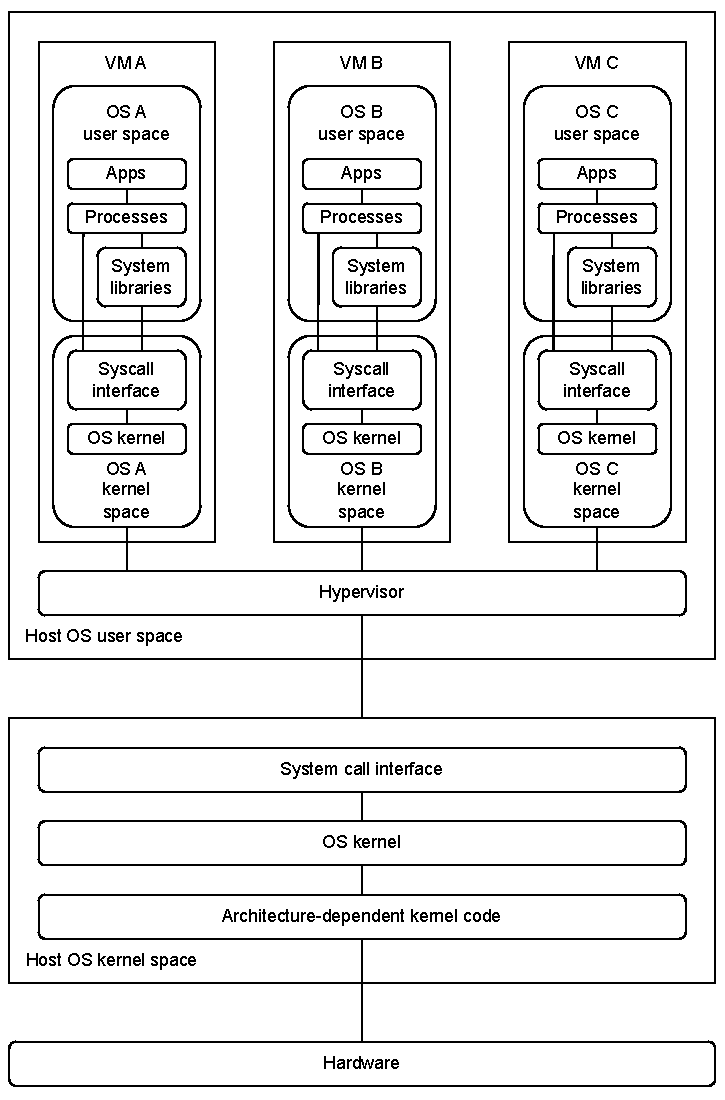
\includegraphics{assets/type_2_virtualization.pdf}
    \caption{Type 2 virtualization environment}
    \label{fig:tipe_2_virtualization}
    \vspace{10pt}
\end{figure}

Figure \ref{fig:bare_metal_virtualization} shows a bare metal virtualization environment. As the name suggests, the hypervisor runs directly on the hardware, implementing an abstraction layer by providing each VM with a virtualized physical hardware representation.
The diagram shows three VMs, each one running a different OS, having a different set of system libraries and running a different set of applications. 

Figure \ref{fig:tipe_2_virtualization} depicts a type 2 virtualization environment.
The hypervisor runs in the host OS user space, providing VMs with access to physical resources by redirecting system calls to the host OS system call interface. Three VMs are shown, each one running a different OS, having a different set of system libraries and running a different set of applications.
In a nutshell, the main difference between type 1 and type 2 virtualization resides in the hypervisor collocation: bare metal hypervisors run directly on the hardware, while type 2 rely on the host OS kernel to access physical resources. For this reason, bare metal virtualization generally provides better performance and better VM isolation than type 2.

\section{Cloud models}
By allowing several VMs to run on the same physical hardware, virtualization technologies allowed the creation of multi-tenant cloud environments. Nowadays, several providers offer VM-based cloud services on a pay-per-use basis, allowing several customers to rent VMs or VM clusters to deploy their applications.
Depending on the degree of customer control over the cloud infrastructure, three main deployment models have emerged: Infrastructure as a Service (IaaS), Platform as a Service (PaaS) and Software as a Service (SaaS) \cite{stonemanLearnDockerMonth}.
Figure \ref{fig:iaas_paas_saas} shows, for each model, which components are managed by cloud providers and which are managed by customers.
According to the IaaS model, cloud providers offer only hardware and basic software resources while customers are responsible for the deployment, management and maintenance of applications.
The PaaS model allows customers to use a complete production environment offered by providers, while the SaaS model provides customers a complete software product, fully functional, already deployed on the cloud and usually accessible through a web browser.
Narrowing the discussion to IaaS and PaaS since SaaS does not allow customers to deploy their own applications, it's worth noting that neither model constitutes an optimal alternative in terms of costs and flexibility.
The IaaS model involves deploying each application component on a separate virtual machine. For this reason, each component must be managed and scaled manually, resulting in expensive and often underutilized VMs. However, this model provides excellent portability between different cloud platforms because the deployment is not cloud-service specific. On the other hand, according to the PaaS model, each component relies on specific cloud services offered by the providers. 
Although more flexible and less expensive than the IaaS model, PaaS deployments are much less portable as they exploit cloud platform-specific services.

\begin{figure}[htbp]
    \vspace{10pt}
    \centering
    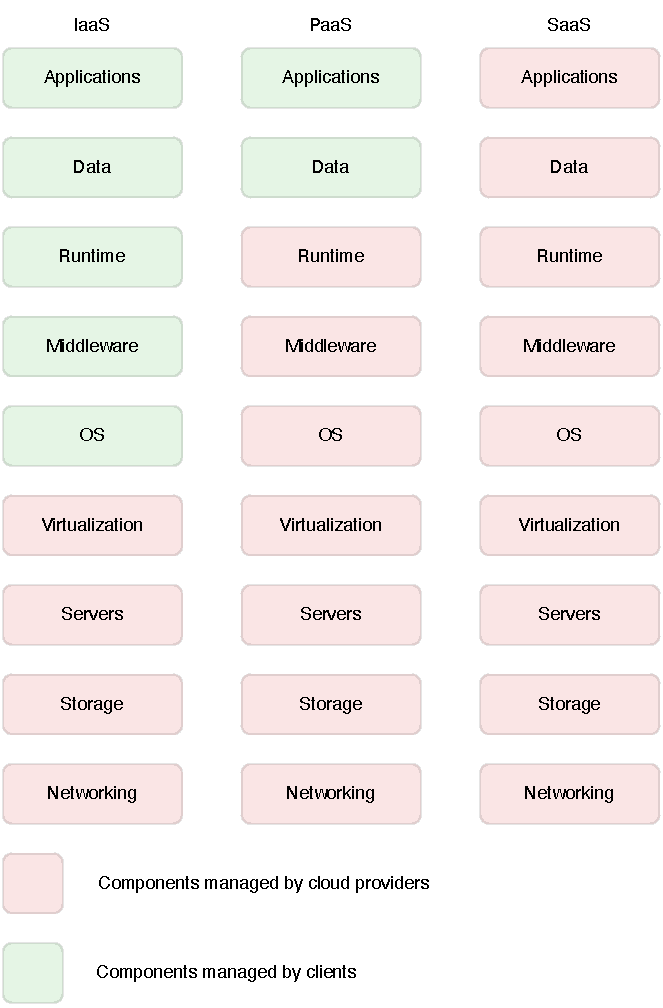
\includegraphics{assets/iaas_paas_saas.pdf}
    \caption{IaaS, PaaS and SaaS cloud models.}
    \label{fig:iaas_paas_saas}
    \vspace{10pt}
\end{figure}
 
\section{Linux containers}
Despite the term container gained popularity after the diffusion of Docker, the technology at its back has been in the engineering landscape since the introduction of Linux Containers (LXC) \cite{LinuxContainers} in 2008. Containers received the attention of the software development community as a lightweight and more flexible alternative to VMs for deploying applications in cloud environments.

A Linux container is a group of Linux processes running in isolation that, unlike VMs, share the same host OS kernel. 
Despite simple from a theoretical perspective, isolating Linux processes in containers is not a trivial task since it requires reliable resource isolation techniques and a software layer capable of using them to group processes. 
The integration in the Linux kernel of \texttt{namespace} and \texttt{cgroups} isolation technologies in 2006 paved the way for the creation of such a layer, making LXC the first example of container runtime, namely a software capable of managing Linux containers by directly interfacing with the underlying host OS Linux kernel.
In other words, LXC provides a user space API (\texttt{liblxc} C system library) that, by using Linux kernel isolation features, allows grouping Linux processes in isolated sets.

Despite being powerful tools, container runtimes alone are not enough to obtain a full functioning containerized environment since they do not provide advanced tools to manage the entire container lifecycle.  
To this purpose, a higher-level software layer is needed, namely a container engine. 
By relying on the container runtime, container engines provide advanced tools for container creation, deletion, orchestration, networking, storage sharing, etc. 

\begin{figure}[htbp]
    \vspace{10pt}
    \centering
    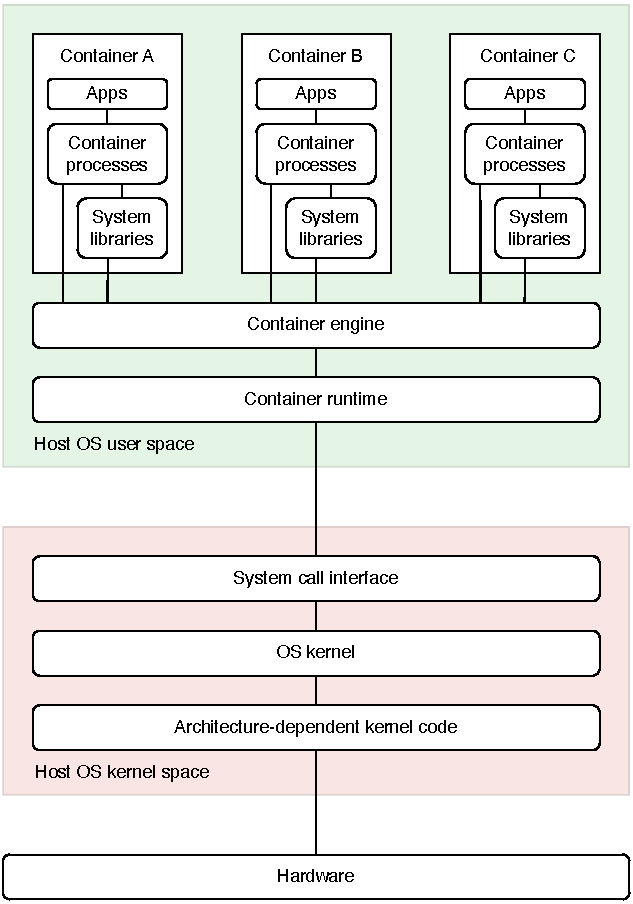
\includegraphics{assets/containerization.pdf}
    \caption{Containerized environment}
    \label{fig:containers}
    \vspace{10pt}
\end{figure}

\newpage
Figure \ref{fig:containers} illustrates a complete containerized environment.
Right above the container engine and runtime layers, the diagram shows three running containers, each one having a different set of system libraries and running a different set of processes in isolation. 
The container engine interfaces with the process layer while the container runtime handles the low-level interaction with the host OS kernel, using system calls to manage \texttt{namespace} and \texttt{cgroups}. 
The host OS kernel space and the hardware layers are depicted as in figure \ref{fig:linux_os_structure}. 

\section{Comparison of Linux containers and virtual machines}
The introduction of Linux containers consisted in a radical departure from traditional virtualization-based deployments, namely IaaS and PaaS: the application is no longer deployed as a monolithic entity on a single VM, but as a set of orchestrated components, each one running in a separate container. 
Container-based deployments address the main problems of traditional IaaS and PaaS models, combining PaaS flexibility with IaaS portability.
Nowadays, modern microservices architectures often follow the Containeer as a Service (CaaS) model, where each application component is deployed in a lightweight, portable and isolated unit.

However, as table \ref{tab:vm_container_comparison} suggests, containers do not play the role of "silver bullets" in the field of software production. 
Containers are usually ephemeral, lightweight and portable wrappers around Linux processes \cite{kaneDockerRunningShipping2023}, 
no more. Virtual machines are an abstraction of physical hardware. 
This difference in philosophy reflects on the use cases of the two technologies. \newline
Virtual machines are often long-lived, with a minimum lifespan of days or weeks. 
For this reason, virtualization is still the solution of choice when a deployment is expected to be long-lived and, in a sense, "stable".
Moreover, virtualization is used when a small set of cloud applications require different operating systems (or different OS versions) \cite{bernstein2014containers}. 
The number of VMs running on a host is usually limited to a few units since each VM consists in a full-fledged OS instance.
Containers are significantly smaller in size: an host can run hundreds or even thousands of containers, each one representing a single application component.
By having lower overhead, higher performance and faster startup and stop times than virtual machines \cite{felter2015updated,chae2019performance}, containers are the perfect solution when the set of services to be deployed is vast but far more homogeneous.
Despite being isolated from each other, the isolation degree of containers is significantly lower than that of virtual machines. While limits can be enforced on the resources containers can access, they usually share CPU and memory on the host system, as co-located UNIX processes do. 

\begin{table}[ht]
    \vspace{10pt}
    \begin{tabularx}{\textwidth}{lXX}
        & VMs & Containers \\
        \midrule
        \textbf{\makecell[l]{Virtualization \\ type}} & Hardware-level & OS-level \\
        \midrule
        \textbf{OS} & Each VM includes a full OS instance running on hypervisor-virtualized hardware & Each container is a set of Linux processes running on the same host OS \\
        \midrule
        \textbf{Overhead} & High & Low \\
        \midrule
        \textbf{Instance size} & $\thicksim$ GB & $\thicksim$ MB \\
        \midrule
        \textbf{Boot time} & $\thicksim$ minutes & $\thicksim$ seconds \\
        \midrule
        \textbf{Lifespan} & $\thicksim$ days or weeks & $\thicksim$ minutes \\
        \midrule
        \textbf{Isolation type} & System-level & Process-level  \\
        \midrule
        \textbf{Security level} & High & Sufficient \\
        \midrule
    \end{tabularx}
    \caption{Comparison of virtual machines and containers}
    \label{tab:vm_container_comparison}
    \vspace{10pt}
\end{table}

\section{Docker}
The introduction of LXC in 2008 was a fundamental step forward the adoption of containerization technologies. However, LXC is only a container runtime, it does not provide advanced tools for managing the entire container lifecycle. \newline
At the time of its first release, on March 20, 2013, Docker provided a container engine that, by using LXC as a container runtime, offered a higher-level API for container management.
On March 13, 2014, with the release of Docker version 0.9, LXC was replaced with a new container runtime, \texttt{libcontainer}, still exploiting Linux kernel isolation features but entirely written in Go.
Nowadays, Docker is way more than a container engine: it's a complete containerization framework that provides a container engine, a container runtime and a set of tools for container sharing and orchestration.
By initially extending LXC and then transitioning to \texttt{libcontainer}, Docker brought Linux containers to the masses, becoming the de-facto standard for containerization. 

\subsection{Docker images and registries}
Container images are the backbone of the entire Docker ecosystem. They are artifacts acting as templates for container instantiation. Images usually contain the OS filesystem, the application component to be deployed and all the dependencies it needs to be run in isolation. 
They are similar to VM templates and may recall Object Oriented Programming classes from which objects (Docker containers) are instantiated.
Their real potential is unleashed when shared between several users and environments through Docker registries, namely public or private repositories where Docker images are made available for download.
The most famous public registry is Docker Hub, an online repository backed by Docker Inc. and sustained by an extensive community of developers. \newline
The addition of images and registries can be considered as the major extension offered by Docker to the LXC technology and the main reason for its widespread adoption.
By pushing and pulling the same image from a registry, developers and operations engineers can create identical containers, ensuring that the application component packed in the image will run consistently on any testing or production environment.
This possibility is crucial in the deployment process since it allows to solve the "it works on my machine" problem, a common issue in software production where the application runs correctly on a particular machine but fails in production due to different configuration or dependencies profiles. 

\subsection{Docker architecture}
Figure \ref{fig:docker_architecture} provides a high-level overview of the Docker architecture. The diagram shows a Docker client, a Docker host and a Docker registry. All these entities can be located on the same physical machine or not. 
The Docker host is the core of the entire architecture, namely the system in which containers are run. By hosting the container engine (daemon) and runtime, the Docker host runs several user-space processes responsible for managing the entire container lifecycle.
The Docker client is a command-line or graphical interface that allows users to interact with the Docker host by sending REST API requests to the docker daemon. A typical Docker workflow foresees developers using a docker client to push a custom image to a registry with \texttt{docker push} and operations engineers to pull the same image with \texttt{docker pull}, later instantiating production containers from it with \texttt{docker run}.
The client-daemon REST API leverages UNIX sockets or network interfaces, depending whether the client and daemon are running on the same machine or not.
The Docker daemon consists of the \texttt{dockerd} process that, by running in the Docker host user space, listens for API requests from Docker clients and manages Docker images, containers, networks and volumes accordingly. 
The Docker container runtime operates at the lowest level, still in the user space. As explained, it interfaces with the host OS kernel to start and stop containers by managing all OS constructs such as \texttt{namespace} and \texttt{cgroups}.
The runtime is implemented in a tiered fashion. The low-level runtime, \texttt{runc}, is the reference implementation of the OCI runtime specification. Its duty is to interface with the underlying Linux host kernel to start and stop containers. The high level runtime, \texttt{containerd}, manages the entire container lifecycle, including pulling images from registries and managing \texttt{runc} instances. \newline
A typical Docker installation has a single \texttt{containerd} process instructing \texttt{runc} to start and stop containers. \texttt{runc} processes are typically short-lived, terminating as soon as a container is started or stopped.
\texttt{dockerd} is located above \texttt{containerd} and performs higher-level tasks such as exposing the Docker REST API, managing images, networks and volumes. 
Docker provides also basic container orchestration tools, such as \texttt{docker-compose} and \texttt{docker swarm}, depicted as the orchestration layer in the figure.

\begin{figure}[htbp]
    \vspace{10pt}
    \centering
    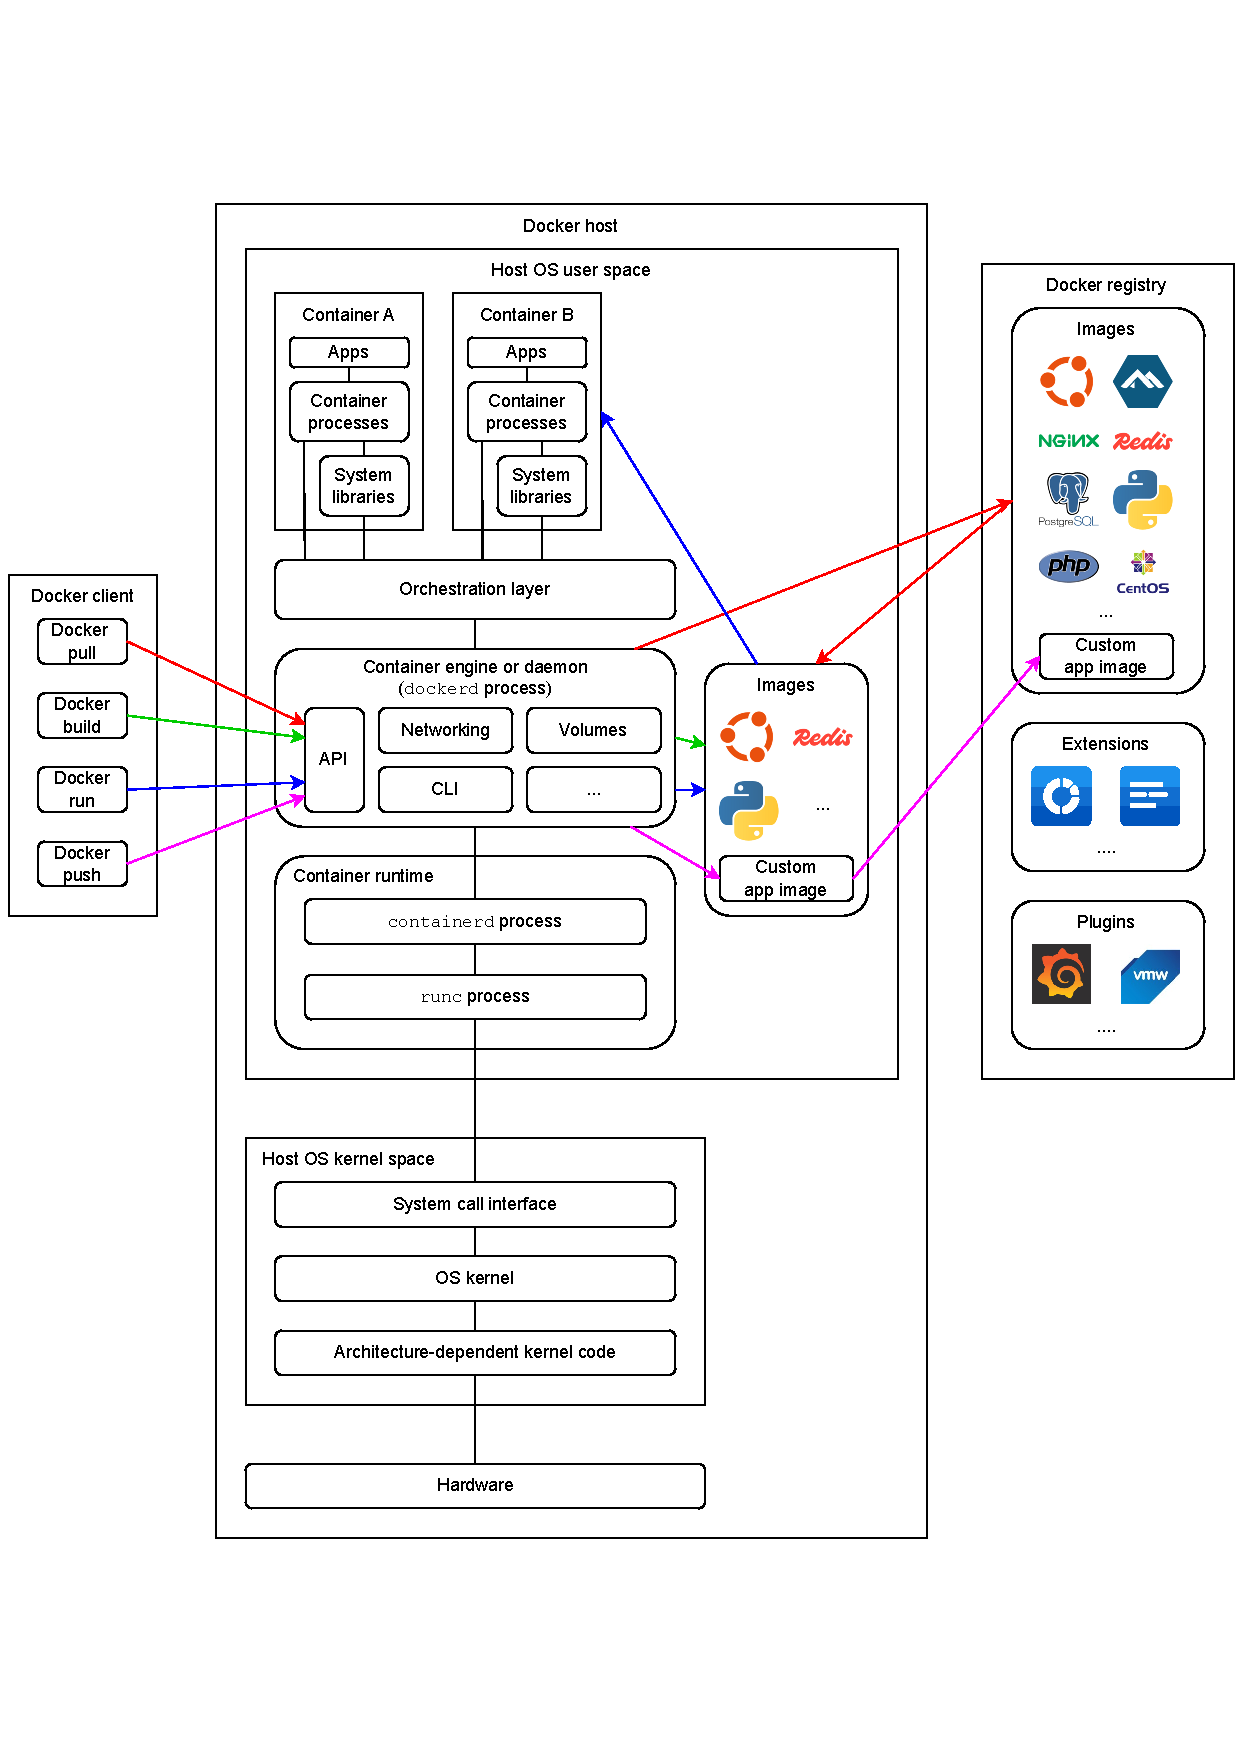
\includegraphics[width=1\textwidth]{assets/docker.pdf}
    \caption{Docker architecture}
    \label{fig:docker_architecture}
    \vspace{10pt}
\end{figure}

\subsection{Single-container application deployment}
With the adoption of Docker, the traditional deployment process described in figure \ref{fig:traditional_deployment} has been radically simplified. The discussion that follows describes each step of an application component deployment while figure \ref{fig:multi_container_deployment} provides a schematic overview of the process.

\begin{enumerate}
    \item Developers test the the application code to be deployed (with all the dependencies it needs) by running it in a containerized testing environment. 
    \item When the application works as expected, Developers create a Dockerfile, namely a text file containing all the instructions needed by the Docker engine to package the application in a Docker image. The Dockerfile usually specifies the base image to be used, where to copy application files, which commands to execute to install dependencies and how to start and run the application.
    \item Developers build the Docker image by using the \texttt{docker build} command and the information contained in the Dockerfile.
    \item Before pushing the image to a Docker registry, developers test the image by instantiating a container from it in a testing environment. Then, they tag the image with a unique identifier by using the \texttt{docker tag} command.
    \item Developers push the image to a Docker registry by using the \texttt{docker push} command.
    \item Operations engineers pull the image from the registry by using the \texttt{docker pull} command, usually specifying its tag. 
    \item Operations engineers instantiate a production container from the image by using the \texttt{docker run} command, providing additional configuration details such as environment variables, network settings, volume mounts, etc.
\end{enumerate}

In a nutshell, developers test the application component by running a container in a testing environment. Once the component is well-tested, it's shared to the operations team using a Docker registry and as a Docker image, then is deployed to production. Both of the two teams can be sure they are dealing with exactly the same artifact, containing the same application component and the same dependencies.
It's worth noting that this description is closer to the typical Docker deployment workflow rather than a real-world deployment process. In such a scenario, the deployment process usually involves creating an automated CI/CD pipeline, from code version control to production deployment. 
Moreover, the distinction between development and operations teams is more nuanced, as the two teams often work together in a DevOps fashion.

\begin{figure}[htbp]
    \vspace{10pt}
    \centering
    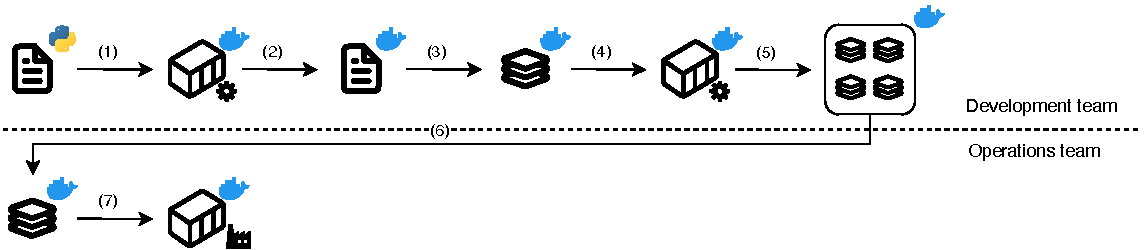
\includegraphics[width=1\textwidth]{assets/single_container_deployment.pdf}
    \caption{Deployment process of a single-container application}
    \label{fig:single_container_deployment}
    \vspace{10pt}
\end{figure}

\subsection{Microservices application deployment}
As discussed in previous sections, complex applications are deployed as a set of microservices, each running in a separate container. This approach allows to scale and update each component independently and aims at providing a higher security level by isolating each service from the others. \newline
The discussion that follows describes each step of a microservices application deployment while figure \ref{fig:multi_container_deployment} provides a schematic overview of the process.
The application to be deployed is composed of three microservices, namely a Python frontend, a Python backend and a MySQL database.  

\begin{enumerate}
    \item Developers test each application component in isolation by running it (with all the dependencies it needs) in a separate containerized testing environment. This phase is close to unit testing. 
    \item When each application component works as expected, Developers create a Dockerfile for each of them.
    \item Developers build a Docker image for each application component by using the \texttt{docker build} command and the information contained in the Dockerfile.
    \item Before pushing each image to a Docker registry, Developers test the entire application by running all its components together, often using tools such as \texttt{docker-compose} to orchestrate the containers. As it involves the interaction between different microservices, this phase is close to integration testing.
    When the application works as expected, developers tag each image with a unique identifier by using the \texttt{docker tag} command.
    \item Developers push the images to a Docker registry by using the \texttt{docker push} command.
    \item Operations engineers pull the images from the registry by using the \texttt{docker pull} command, specifying a tag for each microservice. 
    \item Operations engineers instantiate production containers from the images by using the \texttt{docker run} command. They provide additional configuration details to each service, such as environment variables, network settings, volume mounts, etc. The application is finally deployed by orchestrating the containers, usually orchestration tools like \texttt{docker-compose}\texttt{docker swarm} or Kubernetes.
\end{enumerate}

\begin{figure}[htbp]
    \vspace{10pt}
    \centering
    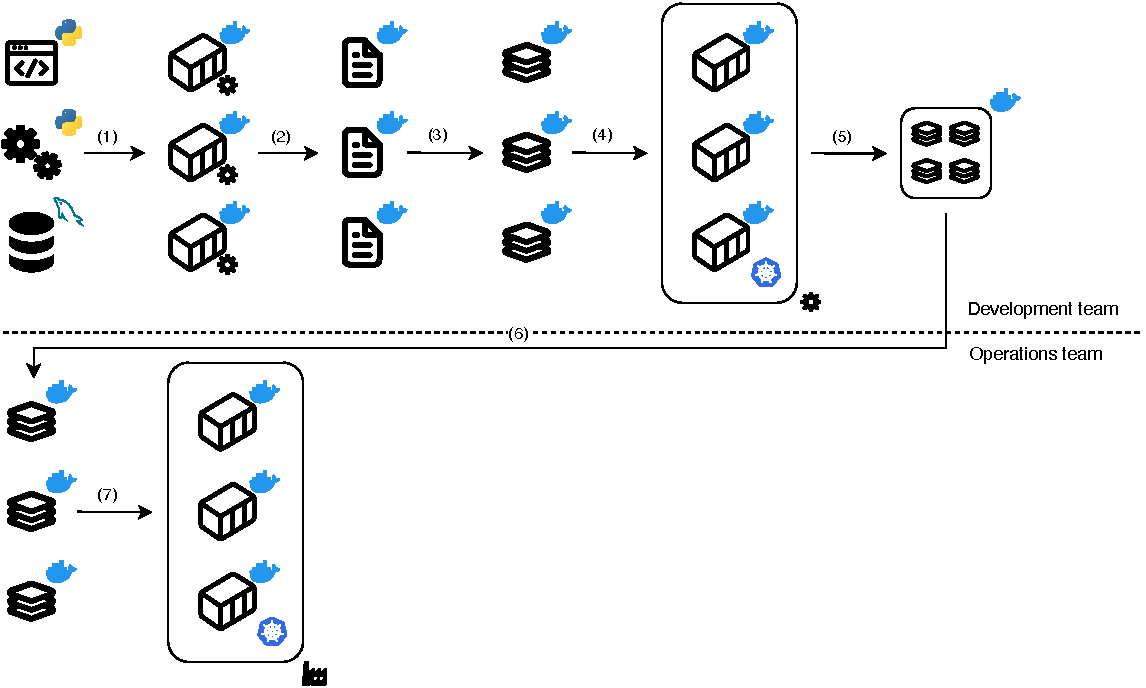
\includegraphics[width=1\textwidth]{assets/multi_container_deployment.pdf}
    \caption{Deployment process of a microservices application}
    \label{fig:multi_container_deployment}
    \vspace{10pt}
\end{figure}

\subsection{Dockerfiles and layered images}
As previously mentioned, Dockerfiles are text files that describe the application component to be deployed and its dependencies in an easy-to-read format \cite{poultonDockerDeepDive2023}. For this reason, they are valuable assets both in application deployment and documentation.

The most evident image feature emerging from  Dockerfiles resides in their layered nature. 
By using Union File Systems (UFS), their file-system exhibit profound differences from a traditional one: images are structured in several layers, each one acting as an immutable "differential filesystem snapshot" with respect to the previous one. Diving into the details, a custom Docker image is created from a base one, namely a minimal Linux distribution (such as Alpine or Ubuntu), acting as layer 0 and containing the clean OS filesystem. Every instruction in the Dockerfile creates a new filesystem layer, encoding the differences between the new filesystem content (or state) and the previous one. For example, layer 1 may differ from layer 0 by containing a new file, layer 2 may differ from layer 1 by containing a new directory, and so on.
This layered structure allows Docker to cache intermediate layers and to share common layers between different images, reducing the overall image storage footprint and speeding up the build process. 
Moreover, layers allow for a finer-grade control over image files: when pushing or pulling images to or from a registry, only the changed layers are transferred, reducing the network overhead and speeding up the entire process. Ultimately, layer's immutability assures that image consistency across all environments, from development to production.

Listing \ref{lst:dockerfile} contains a very simple Dockerfile for packing a Python application in a Docker image. 
Since the Dockerfile contains four instructions, the resulting image will be composed of four layers. With the exception of layer 0, each layer contains only files and directories differing from those in the previous one: layer 1 contains all the updates to the Ubuntu base image, layer 2 the Python installation and layer 3 the application files.

\vspace{10pt}
\begin{lstlisting}[language=Python, caption = Example of a simple Dockerfile, label = lst:dockerfile]
    FROM ubuntu:latest
    RUN apt-get update
    RUN apt-get install -y python3
    COPY ./app /app
\end{lstlisting}
\vspace{10pt}

\subsection{Benefits of Docker}
This section summarizes the main benefits of Docker:
\begin{itemize}
    \item \textbf{Reproducibility and portability}: Due to their layered structure, Docker images are immutable and can be easily shared between different environments. Containers instantiated from the same Docker image run consistently regardless of the host system. 
    As a result, an application component packed in a Docker image runs the same way in a developer's machine, in a testing environment and in production.
    \item \textbf{Isolation}: containers are - or should be - isolated from each other and from the host system, reducing the risk of dependency conflicts between applications and granting a good level of security.
    \item \textbf{Resource efficiency by preserving hardware-software abstraction}: containers share the same host OS kernel. For this reason, containerization exhibit a lower overhead with respect to virtualization. Hardware-software abstraction, usually desired in enterprise solutions, is preserved (to a minor extent compared to virtualization technologies).
    \item \textbf{Scalability}: Docker makes it easier to scale applications, especially if they are deployed by orchestrating microservices. 
    \item \textbf{Low configuration overhead}: Docker simplifies the process of setting up development and production environments, simplifying an error-prone and time-consuming process.
\end{itemize}












